\providecommand{\main}{../../../..}
\documentclass[\main/dresen_thesis.tex]{subfiles}

\begin{document}
  \begin{figure}[tb]
    \centering
    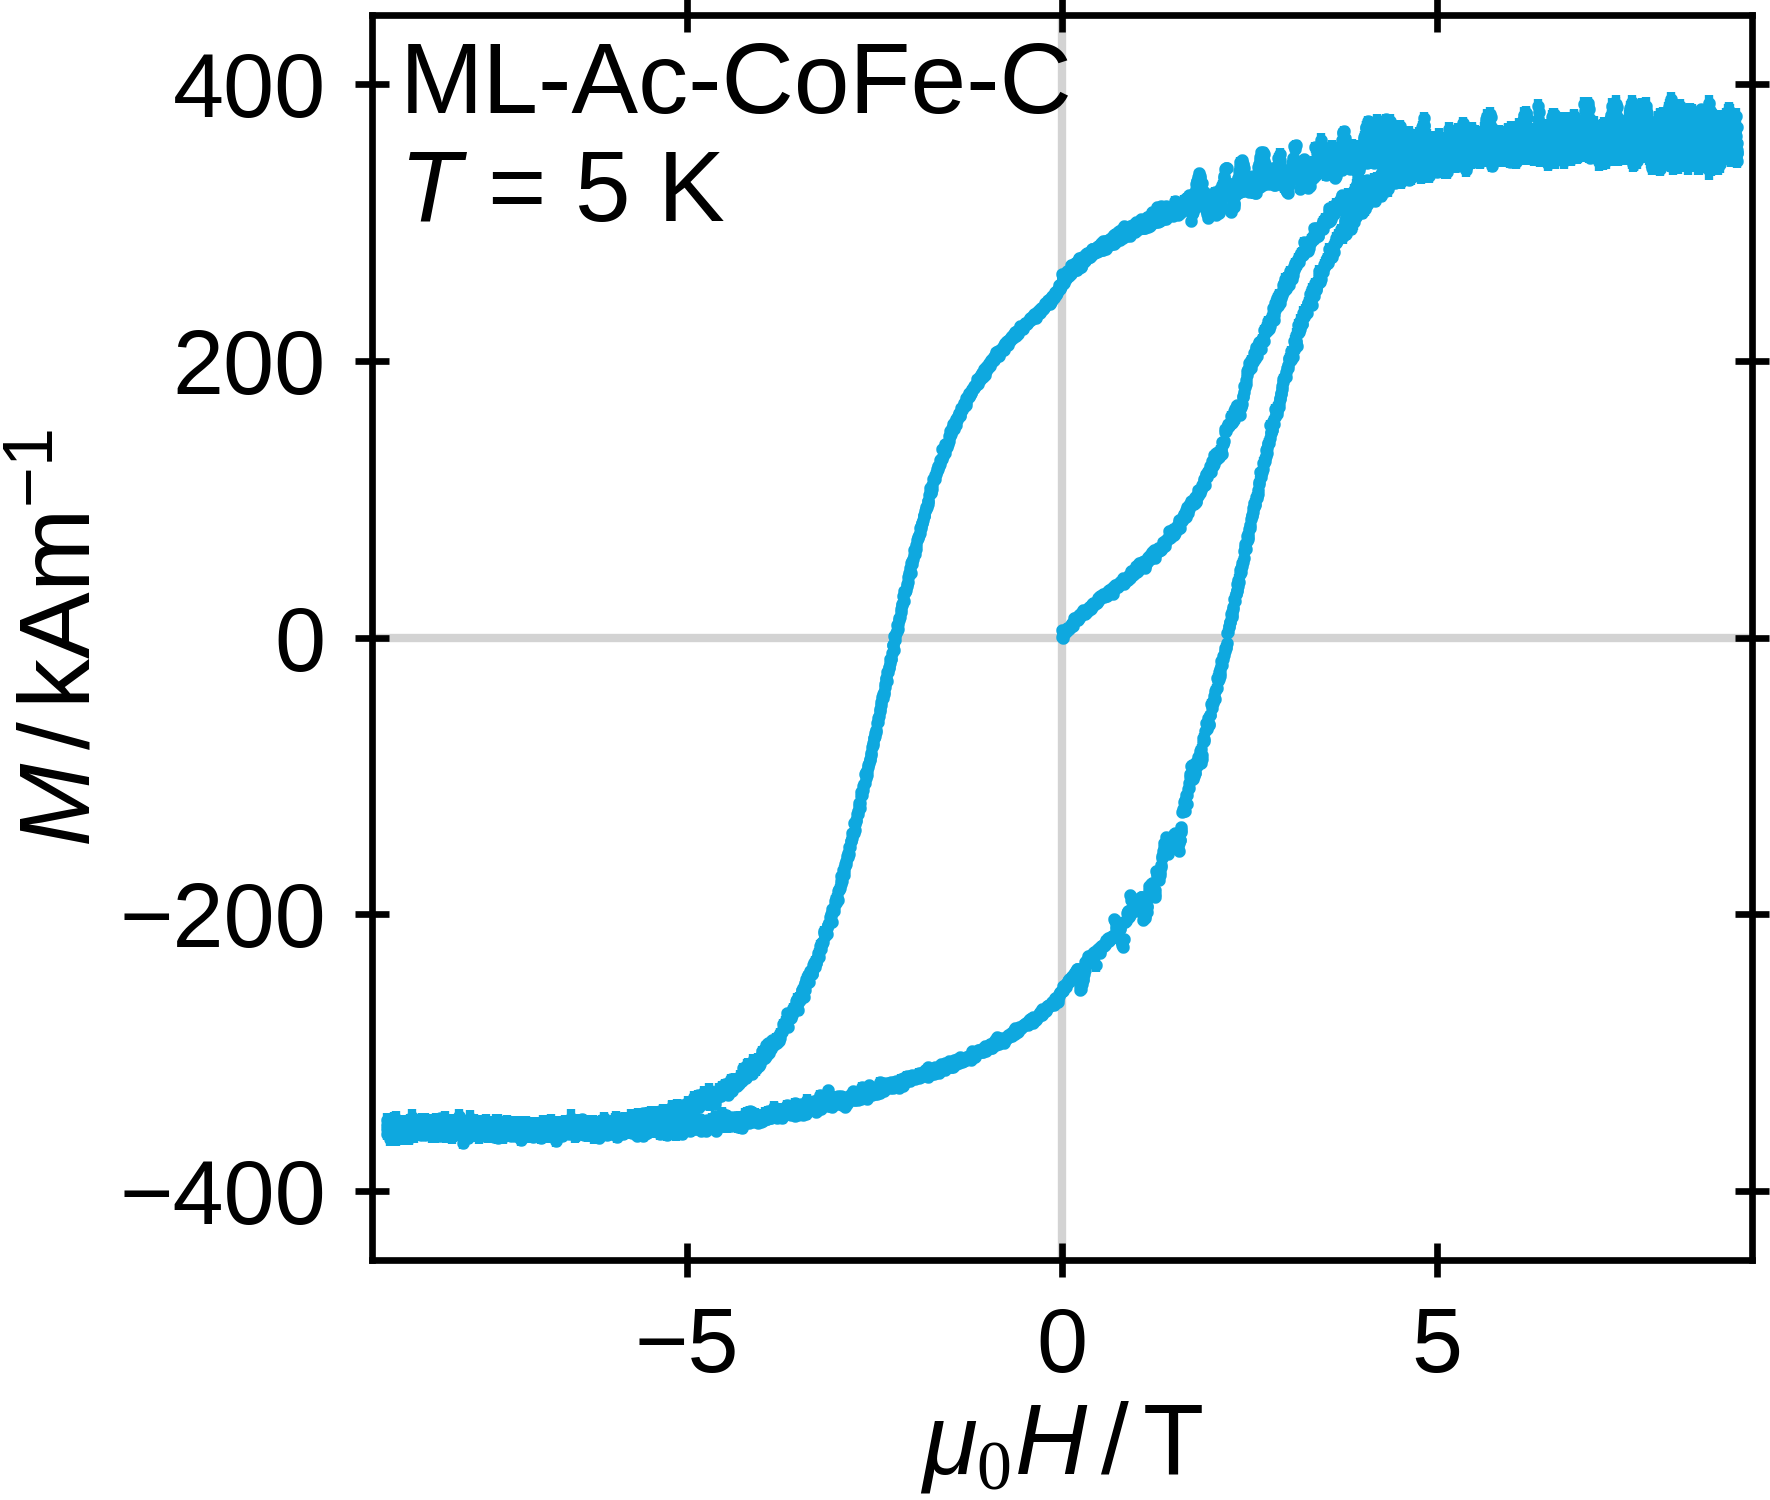
\includegraphics{monolayer_PPMS_VSM_5K_ML_Ac_CoFe_C}
    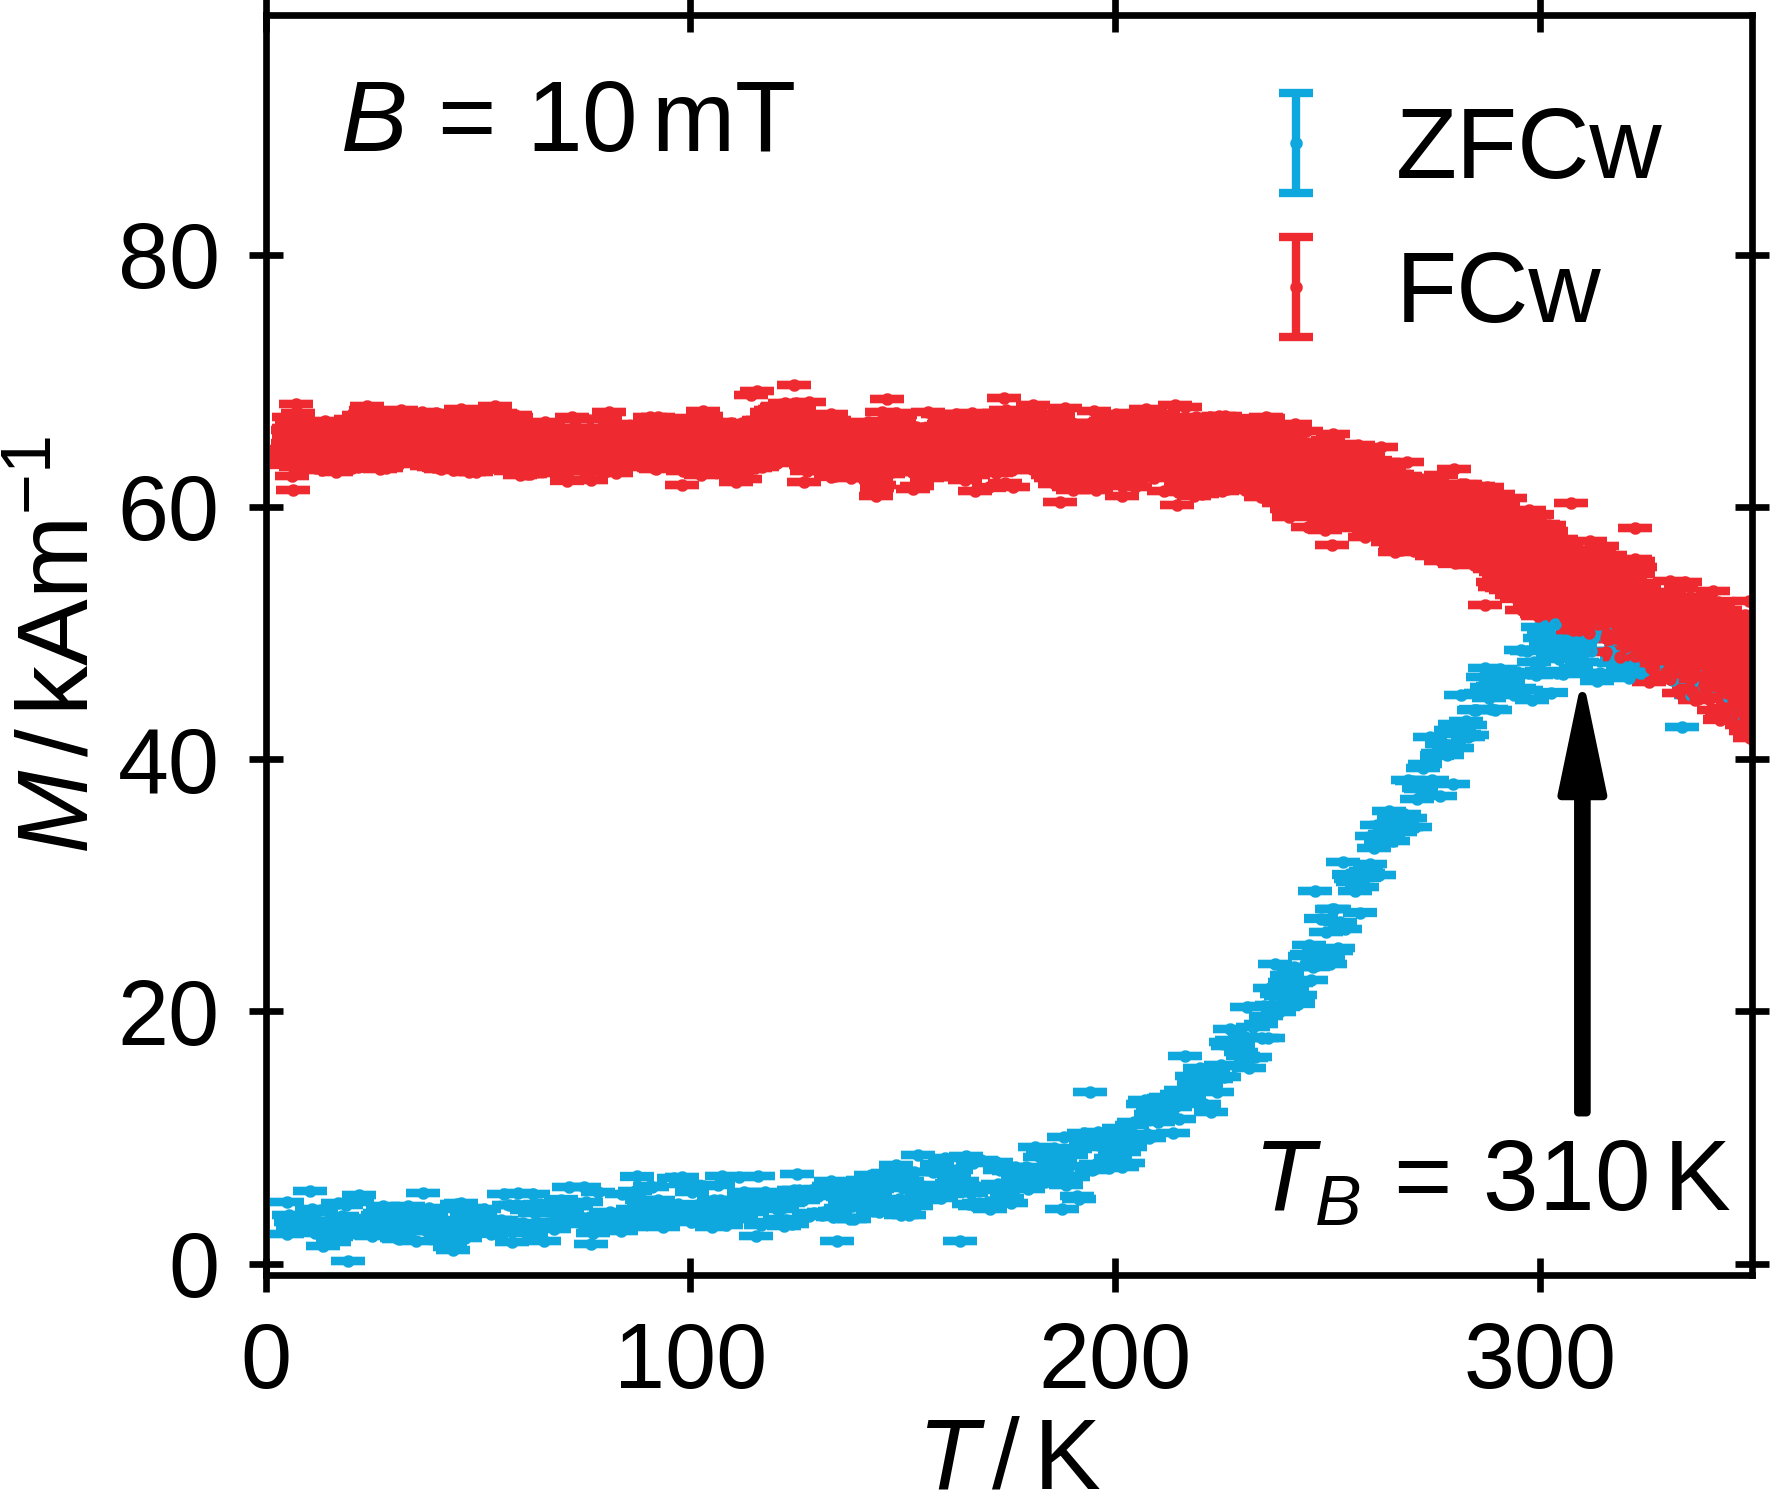
\includegraphics{monolayer_PPMS_ZFC_FC_ML_Ac_CoFe_C}
    \caption{\label{fig:monolayer:magneticStructure:ppms}Low temperature hysteresis (left) and temperature dependent magnetization (right) of ordered monolayer prepared from Ac-CoFe-C.}
  \end{figure}
  After drop casting cubic nanoparticles in a ordered square lattice, the measured low-temperature hysteresis loop changes drastically from the behaviour observed for the unordered case obtained from measuring a frozen dispersion.
  As can be seen in \reffig{fig:monolayer:magneticStructure:ppms} (left), the hysteresis loop shows a strong jump around zero field, which is not visible in the measurement of the same nanoparticles that were frozen in dispersion in \reffig{fig:monolayers:nanoparticle:vsm10K} (right).
  The effect is visible up to a temperature of $150 \unit{K}$ as can be seen in \reffig{fig:monolayer:magneticStructure:ppmsMultiT}.
  % \begin{figure}[tb]
  %   \centering
  %   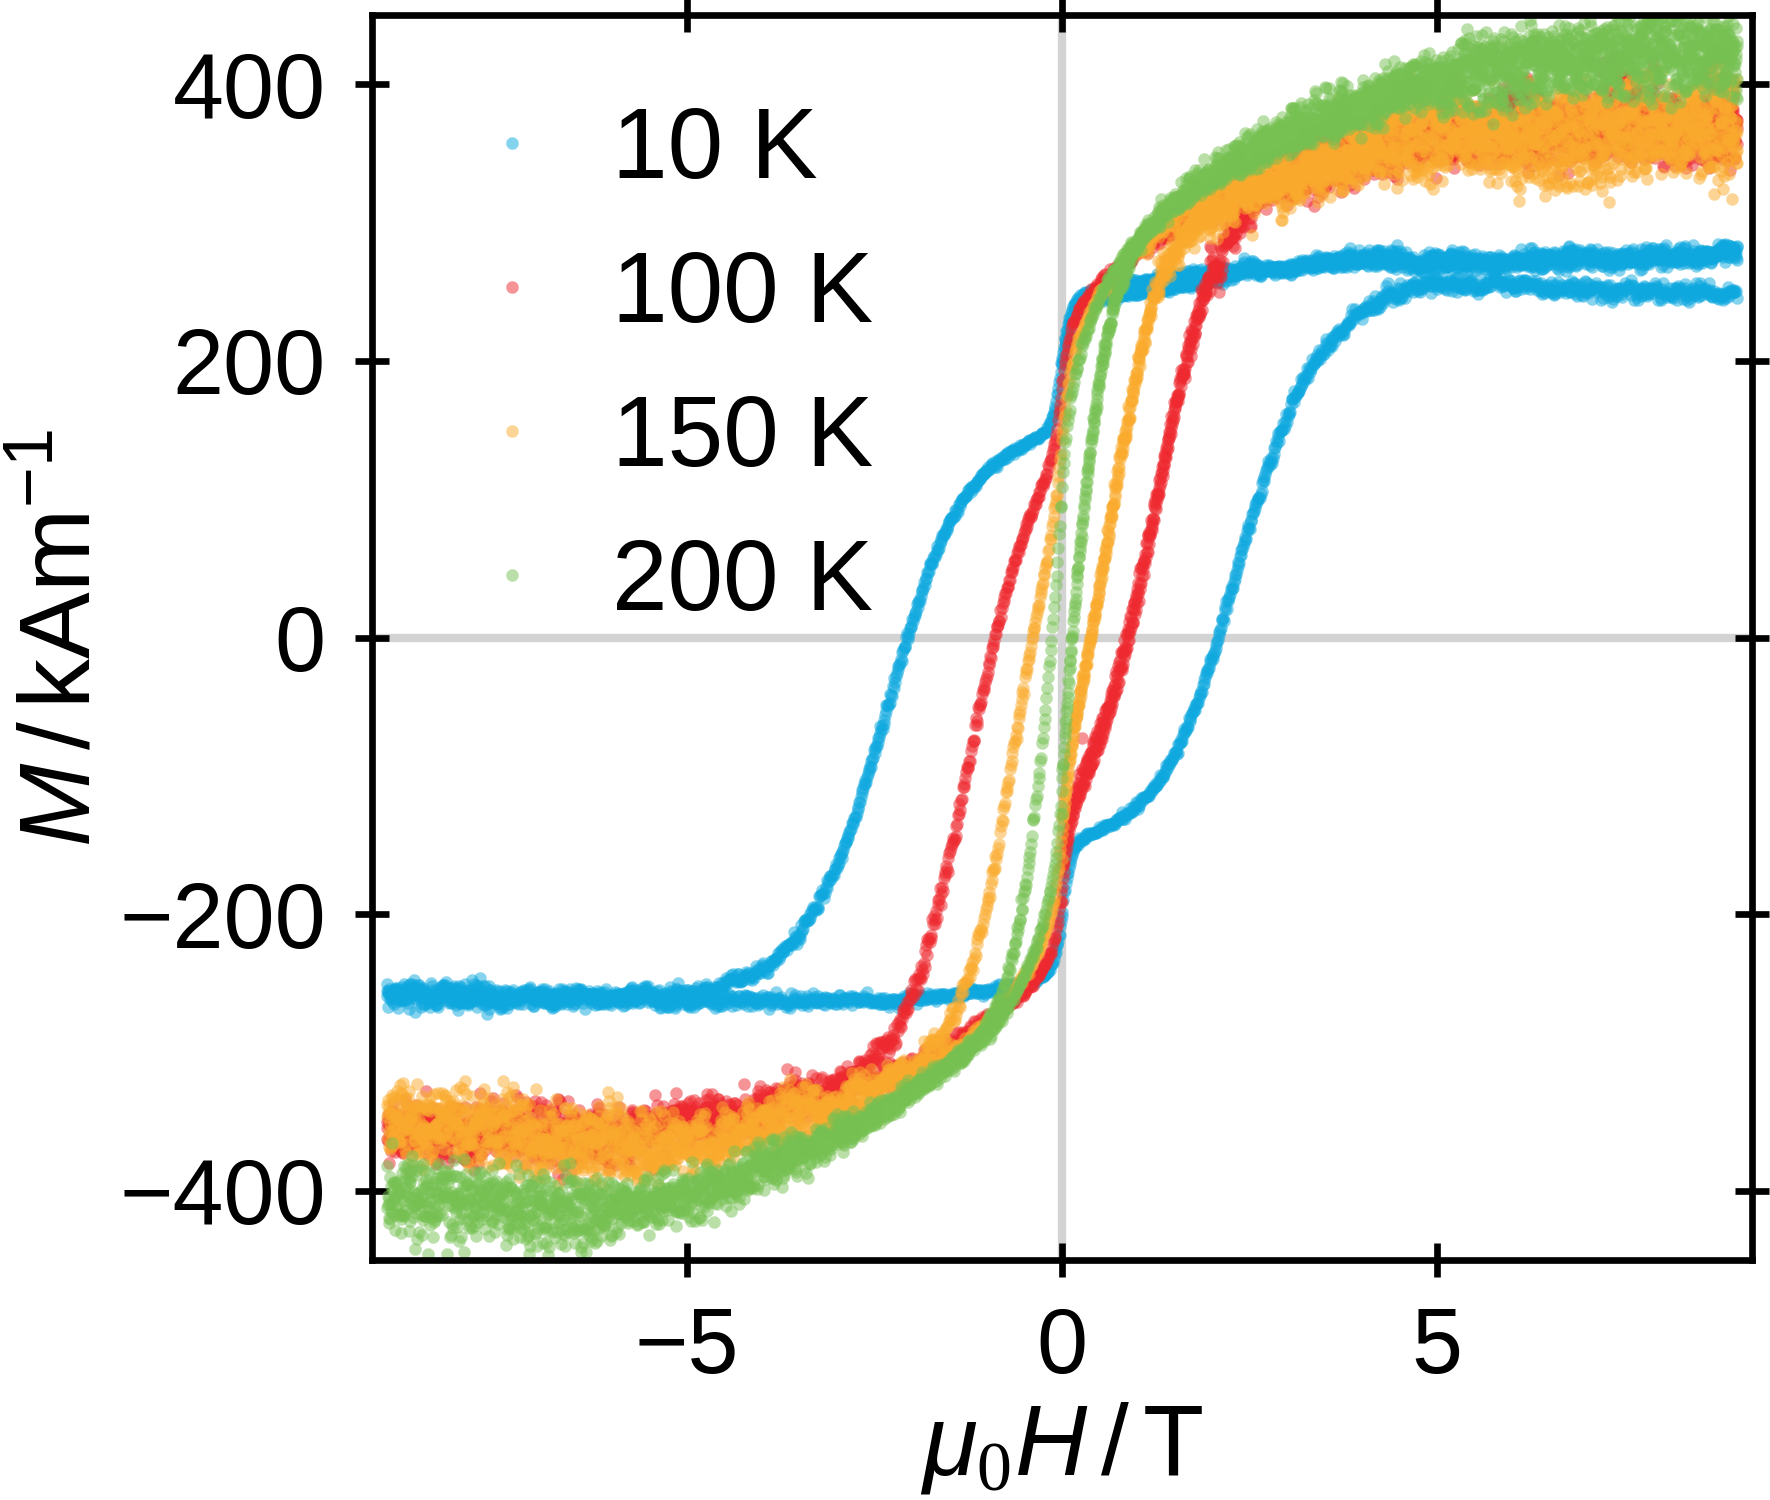
\includegraphics{monolayer_PPMS_VSM_multiTemps_ML_Ac_CoFe_C}
  %   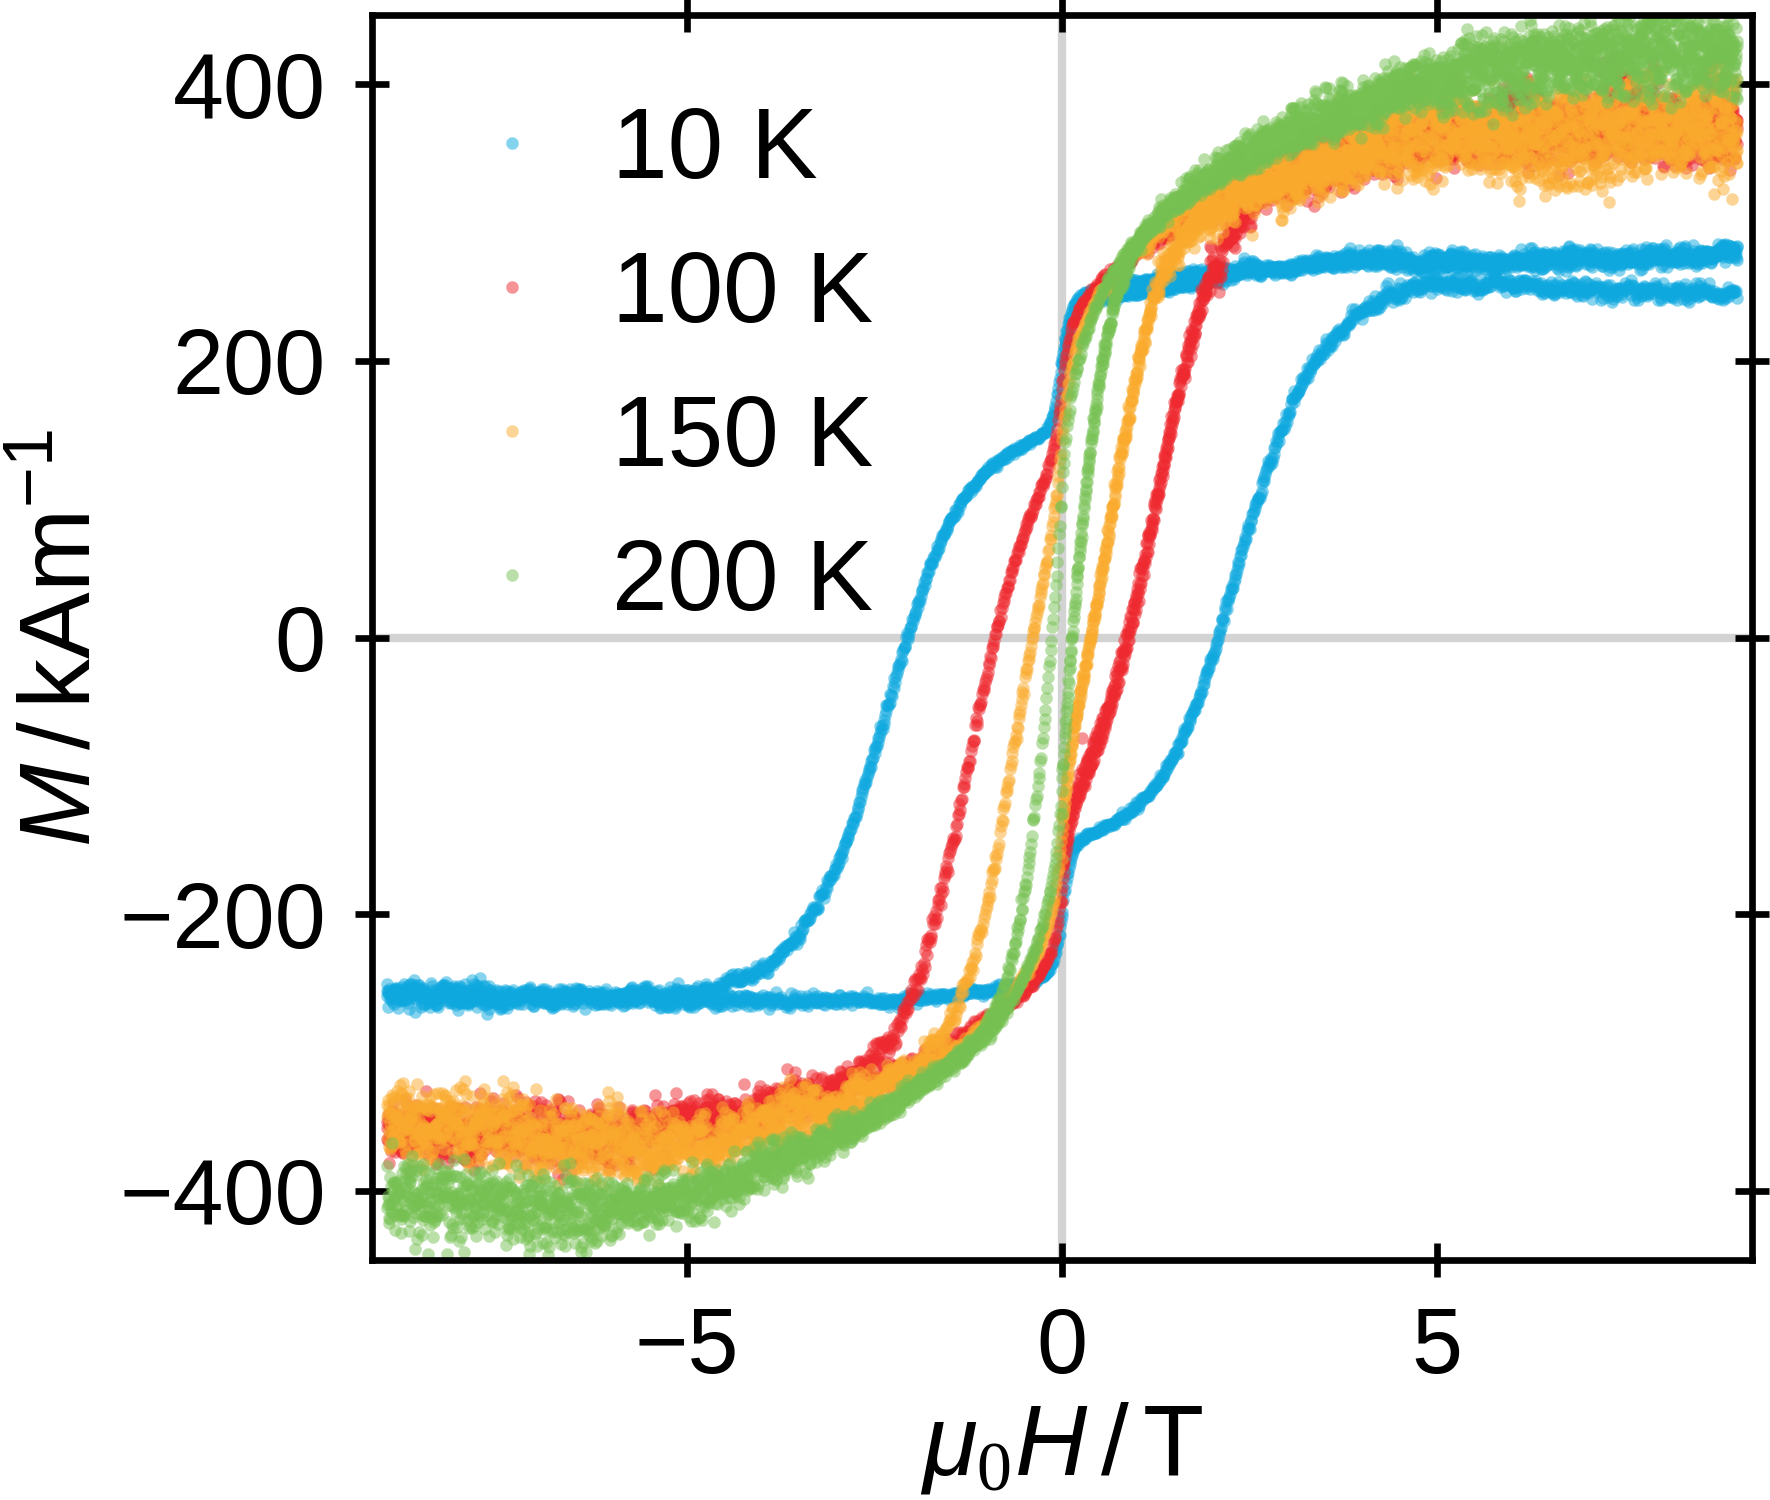
\includegraphics{monolayer_PPMS_VSM_multiTemps_ML_Ac_CoFe_C}
  %   \caption{\label{fig:monolayer:magneticStructure:ppmsMultiT}Magnetic hysteresis measured at multiple temperatures (left).}
  % \end{figure}
\end{document}